\documentclass[twoside]{book}

% Packages required by doxygen
\usepackage{calc}
\usepackage{doxygen}
\usepackage{graphicx}
\usepackage[utf8]{inputenc}
\usepackage{makeidx}
\usepackage{multicol}
\usepackage{multirow}
\usepackage{textcomp}
\usepackage[table]{xcolor}

% Font selection
\usepackage[T1]{fontenc}
\usepackage{mathptmx}
\usepackage[scaled=.90]{helvet}
\usepackage{courier}
\usepackage{amssymb}
\usepackage{sectsty}
\renewcommand{\familydefault}{\sfdefault}
\allsectionsfont{%
  \fontseries{bc}\selectfont%
  \color{darkgray}%
}
\renewcommand{\DoxyLabelFont}{%
  \fontseries{bc}\selectfont%
  \color{darkgray}%
}

% Page & text layout
\usepackage{geometry}
\geometry{%
  a4paper,%
  top=2.5cm,%
  bottom=2.5cm,%
  left=2.5cm,%
  right=2.5cm%
}
\tolerance=750
\hfuzz=15pt
\hbadness=750
\setlength{\emergencystretch}{15pt}
\setlength{\parindent}{0cm}
\setlength{\parskip}{0.2cm}
\makeatletter
\renewcommand{\paragraph}{%
  \@startsection{paragraph}{4}{0ex}{-1.0ex}{1.0ex}{%
    \normalfont\normalsize\bfseries\SS@parafont%
  }%
}
\renewcommand{\subparagraph}{%
  \@startsection{subparagraph}{5}{0ex}{-1.0ex}{1.0ex}{%
    \normalfont\normalsize\bfseries\SS@subparafont%
  }%
}
\makeatother

% Headers & footers
\usepackage{fancyhdr}
\pagestyle{fancyplain}
\fancyhead[LE]{\fancyplain{}{\bfseries\thepage}}
\fancyhead[CE]{\fancyplain{}{}}
\fancyhead[RE]{\fancyplain{}{\bfseries\leftmark}}
\fancyhead[LO]{\fancyplain{}{\bfseries\rightmark}}
\fancyhead[CO]{\fancyplain{}{}}
\fancyhead[RO]{\fancyplain{}{\bfseries\thepage}}
\fancyfoot[LE]{\fancyplain{}{}}
\fancyfoot[CE]{\fancyplain{}{}}
\fancyfoot[RE]{\fancyplain{}{\bfseries\scriptsize Generated on Sat Nov 30 2013 10\-:33\-:47 for Fotoshop by Doxygen }}
\fancyfoot[LO]{\fancyplain{}{\bfseries\scriptsize Generated on Sat Nov 30 2013 10\-:33\-:47 for Fotoshop by Doxygen }}
\fancyfoot[CO]{\fancyplain{}{}}
\fancyfoot[RO]{\fancyplain{}{}}
\renewcommand{\footrulewidth}{0.4pt}
\renewcommand{\chaptermark}[1]{%
  \markboth{#1}{}%
}
\renewcommand{\sectionmark}[1]{%
  \markright{\thesection\ #1}%
}

% Indices & bibliography
\usepackage{natbib}
\usepackage[titles]{tocloft}
\setcounter{tocdepth}{3}
\setcounter{secnumdepth}{5}
\makeindex

% Hyperlinks (required, but should be loaded last)
\usepackage{ifpdf}
\ifpdf
  \usepackage[pdftex,pagebackref=true]{hyperref}
\else
  \usepackage[ps2pdf,pagebackref=true]{hyperref}
\fi
\hypersetup{%
  colorlinks=true,%
  linkcolor=blue,%
  citecolor=blue,%
  unicode%
}

% Custom commands
\newcommand{\clearemptydoublepage}{%
  \newpage{\pagestyle{empty}\cleardoublepage}%
}


%===== C O N T E N T S =====

\begin{document}

% Titlepage & ToC
\hypersetup{pageanchor=false}
\pagenumbering{roman}
\begin{titlepage}
\vspace*{7cm}
\begin{center}%
{\Large Fotoshop }\\
\vspace*{1cm}
{\large Generated by Doxygen 1.8.5}\\
\vspace*{0.5cm}
{\small Sat Nov 30 2013 10:33:47}\\
\end{center}
\end{titlepage}
\clearemptydoublepage
\tableofcontents
\clearemptydoublepage
\pagenumbering{arabic}
\hypersetup{pageanchor=true}

%--- Begin generated contents ---
\chapter{Namespace Index}
\section{Namespace List}
Here is a list of all namespaces with brief descriptions\-:\begin{DoxyCompactList}
\item\contentsline{section}{\hyperlink{namespace_ui}{Ui} \\*Header file for the small new / load / close window }{\pageref{namespace_ui}}{}
\end{DoxyCompactList}

\chapter{Hierarchical Index}
\section{Class Hierarchy}
This inheritance list is sorted roughly, but not completely, alphabetically\-:\begin{DoxyCompactList}
\item Q\-Main\-Window\begin{DoxyCompactList}
\item \contentsline{section}{Main\-Window}{\pageref{class_main_window}}{}
\item \contentsline{section}{workingwindow}{\pageref{classworkingwindow}}{}
\end{DoxyCompactList}
\item \contentsline{section}{undo\-Arr}{\pageref{classundo_arr}}{}
\end{DoxyCompactList}

\chapter{Class Index}
\section{Class List}
Here are the classes, structs, unions and interfaces with brief descriptions\-:\begin{DoxyCompactList}
\item\contentsline{section}{\hyperlink{class_main_window}{Main\-Window} }{\pageref{class_main_window}}{}
\item\contentsline{section}{\hyperlink{classundo_arr}{undo\-Arr} }{\pageref{classundo_arr}}{}
\item\contentsline{section}{\hyperlink{classworkingwindow}{workingwindow} }{\pageref{classworkingwindow}}{}
\end{DoxyCompactList}

\chapter{File Index}
\section{File List}
Here is a list of all files with brief descriptions\-:\begin{DoxyCompactList}
\item\contentsline{section}{C\-:/\-Users/ledio\-\_\-000/\-Documents/\-Git\-Hub/\-C\-S340/\-Fotoshop/\hyperlink{darkroom_8cpp}{darkroom.\-cpp} }{\pageref{darkroom_8cpp}}{}
\item\contentsline{section}{C\-:/\-Users/ledio\-\_\-000/\-Documents/\-Git\-Hub/\-C\-S340/\-Fotoshop/\hyperlink{darkroom_8h}{darkroom.\-h} }{\pageref{darkroom_8h}}{}
\item\contentsline{section}{C\-:/\-Users/ledio\-\_\-000/\-Documents/\-Git\-Hub/\-C\-S340/\-Fotoshop/\hyperlink{filters_8cpp}{filters.\-cpp} \\*C++ code for all of the filter algorithms called in the work area }{\pageref{filters_8cpp}}{}
\item\contentsline{section}{C\-:/\-Users/ledio\-\_\-000/\-Documents/\-Git\-Hub/\-C\-S340/\-Fotoshop/\hyperlink{filters_8h}{filters.\-h} }{\pageref{filters_8h}}{}
\item\contentsline{section}{C\-:/\-Users/ledio\-\_\-000/\-Documents/\-Git\-Hub/\-C\-S340/\-Fotoshop/\hyperlink{includes_8h}{includes.\-h} }{\pageref{includes_8h}}{}
\item\contentsline{section}{C\-:/\-Users/ledio\-\_\-000/\-Documents/\-Git\-Hub/\-C\-S340/\-Fotoshop/\hyperlink{main_8cpp}{main.\-cpp} \\*Main Cpp file for program }{\pageref{main_8cpp}}{}
\item\contentsline{section}{C\-:/\-Users/ledio\-\_\-000/\-Documents/\-Git\-Hub/\-C\-S340/\-Fotoshop/\hyperlink{mainwindow_8cpp}{mainwindow.\-cpp} \\*Holds the code that is initially run to output the first G\-U\-I window }{\pageref{mainwindow_8cpp}}{}
\item\contentsline{section}{C\-:/\-Users/ledio\-\_\-000/\-Documents/\-Git\-Hub/\-C\-S340/\-Fotoshop/\hyperlink{mainwindow_8h}{mainwindow.\-h} }{\pageref{mainwindow_8h}}{}
\item\contentsline{section}{C\-:/\-Users/ledio\-\_\-000/\-Documents/\-Git\-Hub/\-C\-S340/\-Fotoshop/\hyperlink{_undo_array_8cpp}{Undo\-Array.\-cpp} }{\pageref{_undo_array_8cpp}}{}
\item\contentsline{section}{C\-:/\-Users/ledio\-\_\-000/\-Documents/\-Git\-Hub/\-C\-S340/\-Fotoshop/\hyperlink{workingwindow_8cpp}{workingwindow.\-cpp} }{\pageref{workingwindow_8cpp}}{}
\item\contentsline{section}{C\-:/\-Users/ledio\-\_\-000/\-Documents/\-Git\-Hub/\-C\-S340/\-Fotoshop/\hyperlink{workingwindow_8h}{workingwindow.\-h} }{\pageref{workingwindow_8h}}{}
\end{DoxyCompactList}

\chapter{Namespace Documentation}
\hypertarget{namespace_ui}{\section{Ui Namespace Reference}
\label{namespace_ui}\index{Ui@{Ui}}
}


the header file for the small new / load / close window  




\subsection{Detailed Description}
the header file for the small new / load / close window \hyperlink{class_main_window}{Main\-Window} 
\chapter{Class Documentation}
\hypertarget{class_main_window}{\section{Main\-Window Class Reference}
\label{class_main_window}\index{Main\-Window@{Main\-Window}}
}


{\ttfamily \#include $<$mainwindow.\-h$>$}

Inheritance diagram for Main\-Window\-:\begin{figure}[H]
\begin{center}
\leavevmode
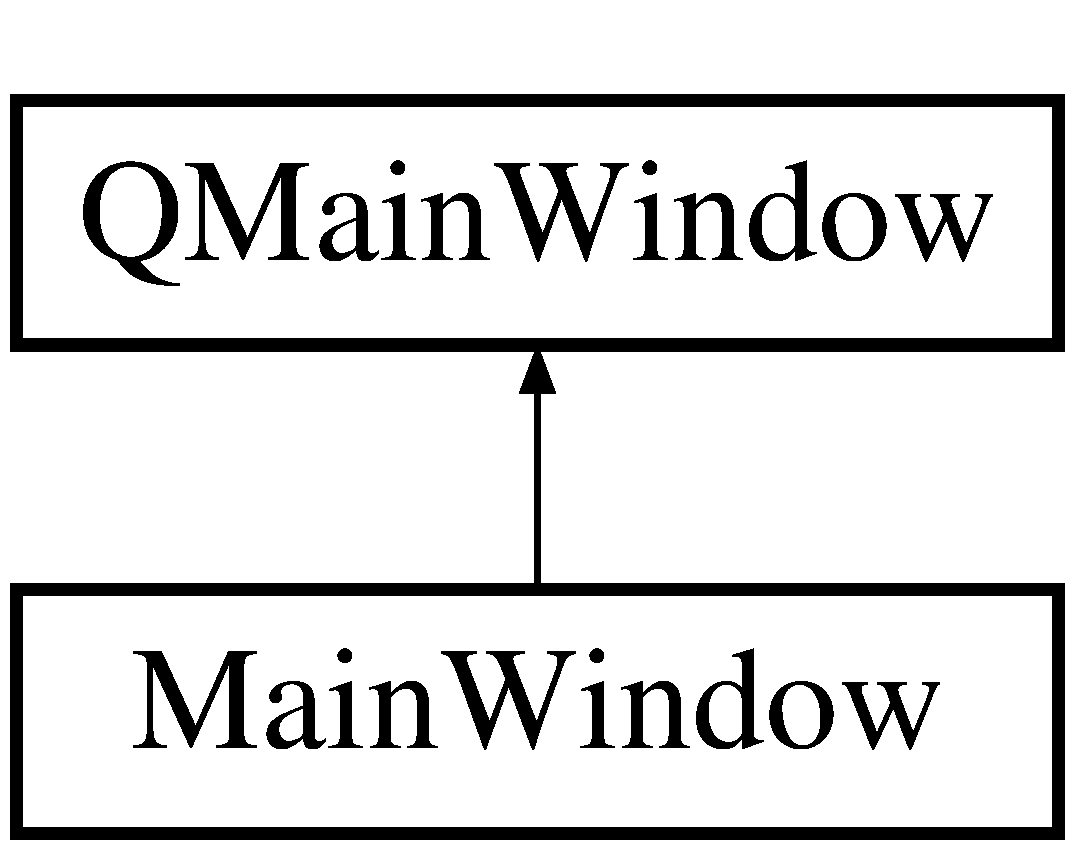
\includegraphics[height=2.000000cm]{class_main_window}
\end{center}
\end{figure}
\subsection*{Public Member Functions}
\begin{DoxyCompactItemize}
\item 
\hyperlink{class_main_window_a8b244be8b7b7db1b08de2a2acb9409db}{Main\-Window} (Q\-Widget $\ast$parent=0)
\item 
\hyperlink{class_main_window_ae98d00a93bc118200eeef9f9bba1dba7}{$\sim$\-Main\-Window} ()
\end{DoxyCompactItemize}


\subsection{Detailed Description}


Definition at line 12 of file mainwindow.\-h.



\subsection{Constructor \& Destructor Documentation}
\hypertarget{class_main_window_a8b244be8b7b7db1b08de2a2acb9409db}{\index{Main\-Window@{Main\-Window}!Main\-Window@{Main\-Window}}
\index{Main\-Window@{Main\-Window}!MainWindow@{Main\-Window}}
\subsubsection[{Main\-Window}]{\setlength{\rightskip}{0pt plus 5cm}Main\-Window\-::\-Main\-Window (
\begin{DoxyParamCaption}
\item[{Q\-Widget $\ast$}]{parent = {\ttfamily 0}}
\end{DoxyParamCaption}
)\hspace{0.3cm}{\ttfamily [explicit]}}}\label{class_main_window_a8b244be8b7b7db1b08de2a2acb9409db}


Definition at line 7 of file mainwindow.\-cpp.

\hypertarget{class_main_window_ae98d00a93bc118200eeef9f9bba1dba7}{\index{Main\-Window@{Main\-Window}!$\sim$\-Main\-Window@{$\sim$\-Main\-Window}}
\index{$\sim$\-Main\-Window@{$\sim$\-Main\-Window}!MainWindow@{Main\-Window}}
\subsubsection[{$\sim$\-Main\-Window}]{\setlength{\rightskip}{0pt plus 5cm}Main\-Window\-::$\sim$\-Main\-Window (
\begin{DoxyParamCaption}
{}
\end{DoxyParamCaption}
)}}\label{class_main_window_ae98d00a93bc118200eeef9f9bba1dba7}


Definition at line 14 of file mainwindow.\-cpp.



The documentation for this class was generated from the following files\-:\begin{DoxyCompactItemize}
\item 
C\-:/\-Users/ledio\-\_\-000/\-Documents/\-Git\-Hub/\-C\-S340/\-Fotoshop/\hyperlink{mainwindow_8h}{mainwindow.\-h}\item 
C\-:/\-Users/ledio\-\_\-000/\-Documents/\-Git\-Hub/\-C\-S340/\-Fotoshop/\hyperlink{mainwindow_8cpp}{mainwindow.\-cpp}\end{DoxyCompactItemize}

\hypertarget{classundo_arr}{\section{undo\-Arr Class Reference}
\label{classundo_arr}\index{undo\-Arr@{undo\-Arr}}
}


{\ttfamily \#include $<$includes.\-h$>$}

\subsection*{Public Member Functions}
\begin{DoxyCompactItemize}
\item 
void \hyperlink{classundo_arr_a55d5c4487ef355fa732fa6db7d57855d}{push} (Q\-Image file)
\item 
void \hyperlink{classundo_arr_a16c74ec4a7e73d8852d634c190bcd51c}{pop} ()
\end{DoxyCompactItemize}
\subsection*{Public Attributes}
\begin{DoxyCompactItemize}
\item 
Q\-Image \hyperlink{classundo_arr_ac8927631ec42f0f4a56ccd66dfbfc732}{curr\-Img}
\item 
bool \hyperlink{classundo_arr_a73c53d3302242f3b5f2e504d9a79fde7}{has\-Pic}
\item 
int \hyperlink{classundo_arr_a01b2d58c78f87f57f163702f565731a2}{size}
\end{DoxyCompactItemize}


\subsection{Detailed Description}
Undo Class 

Definition at line 55 of file includes.\-h.



\subsection{Member Function Documentation}
\hypertarget{classundo_arr_a16c74ec4a7e73d8852d634c190bcd51c}{\index{undo\-Arr@{undo\-Arr}!pop@{pop}}
\index{pop@{pop}!undoArr@{undo\-Arr}}
\subsubsection[{pop}]{\setlength{\rightskip}{0pt plus 5cm}void undo\-Arr\-::pop (
\begin{DoxyParamCaption}
{}
\end{DoxyParamCaption}
)}}\label{classundo_arr_a16c74ec4a7e73d8852d634c190bcd51c}
\hypertarget{classundo_arr_a55d5c4487ef355fa732fa6db7d57855d}{\index{undo\-Arr@{undo\-Arr}!push@{push}}
\index{push@{push}!undoArr@{undo\-Arr}}
\subsubsection[{push}]{\setlength{\rightskip}{0pt plus 5cm}void undo\-Arr\-::push (
\begin{DoxyParamCaption}
\item[{Q\-Image}]{file}
\end{DoxyParamCaption}
)}}\label{classundo_arr_a55d5c4487ef355fa732fa6db7d57855d}


Definition at line 6 of file Undo\-Array.\-cpp.



\subsection{Member Data Documentation}
\hypertarget{classundo_arr_ac8927631ec42f0f4a56ccd66dfbfc732}{\index{undo\-Arr@{undo\-Arr}!curr\-Img@{curr\-Img}}
\index{curr\-Img@{curr\-Img}!undoArr@{undo\-Arr}}
\subsubsection[{curr\-Img}]{\setlength{\rightskip}{0pt plus 5cm}Q\-Image undo\-Arr\-::curr\-Img}}\label{classundo_arr_ac8927631ec42f0f4a56ccd66dfbfc732}


Definition at line 59 of file includes.\-h.

\hypertarget{classundo_arr_a73c53d3302242f3b5f2e504d9a79fde7}{\index{undo\-Arr@{undo\-Arr}!has\-Pic@{has\-Pic}}
\index{has\-Pic@{has\-Pic}!undoArr@{undo\-Arr}}
\subsubsection[{has\-Pic}]{\setlength{\rightskip}{0pt plus 5cm}bool undo\-Arr\-::has\-Pic}}\label{classundo_arr_a73c53d3302242f3b5f2e504d9a79fde7}


Definition at line 60 of file includes.\-h.

\hypertarget{classundo_arr_a01b2d58c78f87f57f163702f565731a2}{\index{undo\-Arr@{undo\-Arr}!size@{size}}
\index{size@{size}!undoArr@{undo\-Arr}}
\subsubsection[{size}]{\setlength{\rightskip}{0pt plus 5cm}int undo\-Arr\-::size}}\label{classundo_arr_a01b2d58c78f87f57f163702f565731a2}


Definition at line 63 of file includes.\-h.



The documentation for this class was generated from the following files\-:\begin{DoxyCompactItemize}
\item 
C\-:/\-Users/ledio\-\_\-000/\-Documents/\-Git\-Hub/\-C\-S340/\-Fotoshop/\hyperlink{includes_8h}{includes.\-h}\item 
C\-:/\-Users/ledio\-\_\-000/\-Documents/\-Git\-Hub/\-C\-S340/\-Fotoshop/\hyperlink{_undo_array_8cpp}{Undo\-Array.\-cpp}\end{DoxyCompactItemize}

\hypertarget{classworkingwindow}{\section{workingwindow Class Reference}
\label{classworkingwindow}\index{workingwindow@{workingwindow}}
}


{\ttfamily \#include $<$workingwindow.\-h$>$}

Inheritance diagram for workingwindow\-:\begin{figure}[H]
\begin{center}
\leavevmode
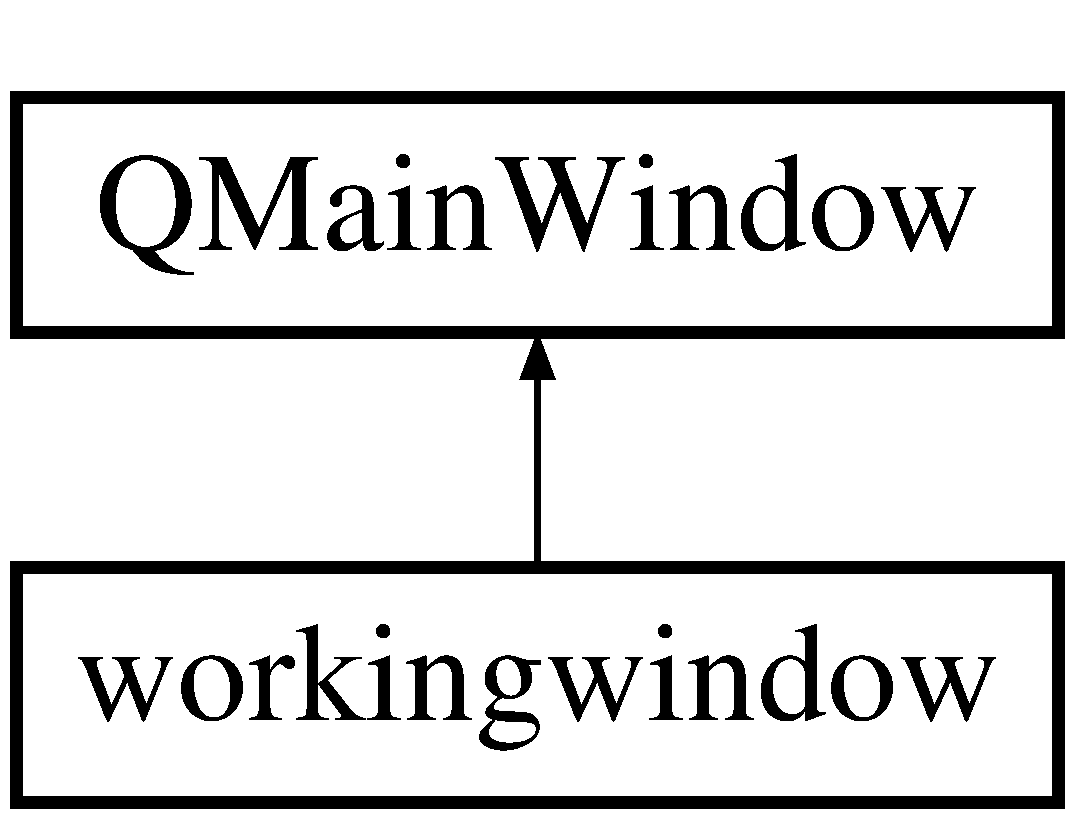
\includegraphics[height=2.000000cm]{classworkingwindow}
\end{center}
\end{figure}
\subsection*{Public Member Functions}
\begin{DoxyCompactItemize}
\item 
\hyperlink{classworkingwindow_a25b4ff6fe8b8cce836be4a4704132a68}{workingwindow} (Q\-Widget $\ast$parent=0)
\item 
\hyperlink{classworkingwindow_a0da6e75e764e958f1267c47dc4edf53c}{$\sim$workingwindow} ()
\end{DoxyCompactItemize}
\subsection*{Public Attributes}
\begin{DoxyCompactItemize}
\item 
Q\-Image \hyperlink{classworkingwindow_ab9ed1f2dafd42f388fc7b366d25db626}{Color\-Wheel}
\item 
bool \hyperlink{classworkingwindow_ab1e5dc3b626cb9e28983e6abee34d10d}{color\-Sampler}
\begin{DoxyCompactList}\small\item\em color\-Wheel for reference in the U\-I \end{DoxyCompactList}\item 
double \hyperlink{classworkingwindow_aee9919c1cfad4526c7b66c5f09b8ce02}{color\-Factor}
\item 
Q\-Color \hyperlink{classworkingwindow_a44fa7af5c036e2686e55c31a3b69e81f}{custom\-Color}
\item 
Q\-Image \hyperlink{classworkingwindow_a470b6dd89240fb31393ee848cef5a358}{color\-Preview}
\item 
bool \hyperlink{classworkingwindow_a48d7fd2e19079e21a8474ae0519f0862}{bucket}
\begin{DoxyCompactList}\small\item\em a window to display the current color selection \end{DoxyCompactList}\item 
Q\-Point \hyperlink{classworkingwindow_aa0c6e8030d9bb3b26324aaf737f2be62}{Static\-X\-Y}
\item 
Q\-Point \hyperlink{classworkingwindow_a0574618dfbe458eee7fac25620c2cf89}{Static\-X\-Y2}
\item 
double \hyperlink{classworkingwindow_a9e3b2de905cba0520347811c530958da}{left\-Line\-Pos}
\item 
double \hyperlink{classworkingwindow_ad140ff2651f5e7993503d5d862e4d385}{right\-Line\-Pos}
\item 
double \hyperlink{classworkingwindow_a1d4abbc294787013faaa0b6f2ee25a2d}{top\-Line\-Pos}
\item 
double \hyperlink{classworkingwindow_a122ed0dce6353c78902353ceeda6bee0}{bottom\-Line\-Pos}
\end{DoxyCompactItemize}


\subsection{Detailed Description}


Definition at line 19 of file workingwindow.\-h.



\subsection{Constructor \& Destructor Documentation}
\hypertarget{classworkingwindow_a25b4ff6fe8b8cce836be4a4704132a68}{\index{workingwindow@{workingwindow}!workingwindow@{workingwindow}}
\index{workingwindow@{workingwindow}!workingwindow@{workingwindow}}
\subsubsection[{workingwindow}]{\setlength{\rightskip}{0pt plus 5cm}workingwindow\-::workingwindow (
\begin{DoxyParamCaption}
\item[{Q\-Widget $\ast$}]{parent = {\ttfamily 0}}
\end{DoxyParamCaption}
)\hspace{0.3cm}{\ttfamily [explicit]}}}\label{classworkingwindow_a25b4ff6fe8b8cce836be4a4704132a68}
creating a proxy to edit with

create a blank white image at 1600 x 900

fill it in blank white

set a blank Qlabel for ui design

fill the blank label with black

set a multiplier so sliders represent color values

set horizontal slider position

set second horizontal slider position

set first vertical slider position

set second vertical slider position

set an image as a color wheel for reference

scale the color wheel to fit the window

push the initial picture to the base of the stack

smooth out pen lines

round out the pen cap 

Definition at line 8 of file workingwindow.\-cpp.

\hypertarget{classworkingwindow_a0da6e75e764e958f1267c47dc4edf53c}{\index{workingwindow@{workingwindow}!$\sim$workingwindow@{$\sim$workingwindow}}
\index{$\sim$workingwindow@{$\sim$workingwindow}!workingwindow@{workingwindow}}
\subsubsection[{$\sim$workingwindow}]{\setlength{\rightskip}{0pt plus 5cm}workingwindow\-::$\sim$workingwindow (
\begin{DoxyParamCaption}
{}
\end{DoxyParamCaption}
)}}\label{classworkingwindow_a0da6e75e764e958f1267c47dc4edf53c}


Definition at line 67 of file workingwindow.\-cpp.



\subsection{Member Data Documentation}
\hypertarget{classworkingwindow_a122ed0dce6353c78902353ceeda6bee0}{\index{workingwindow@{workingwindow}!bottom\-Line\-Pos@{bottom\-Line\-Pos}}
\index{bottom\-Line\-Pos@{bottom\-Line\-Pos}!workingwindow@{workingwindow}}
\subsubsection[{bottom\-Line\-Pos}]{\setlength{\rightskip}{0pt plus 5cm}double workingwindow\-::bottom\-Line\-Pos}}\label{classworkingwindow_a122ed0dce6353c78902353ceeda6bee0}


Definition at line 41 of file workingwindow.\-h.

\hypertarget{classworkingwindow_a48d7fd2e19079e21a8474ae0519f0862}{\index{workingwindow@{workingwindow}!bucket@{bucket}}
\index{bucket@{bucket}!workingwindow@{workingwindow}}
\subsubsection[{bucket}]{\setlength{\rightskip}{0pt plus 5cm}bool workingwindow\-::bucket}}\label{classworkingwindow_a48d7fd2e19079e21a8474ae0519f0862}


a window to display the current color selection 

color\-Preview 

Definition at line 37 of file workingwindow.\-h.

\hypertarget{classworkingwindow_aee9919c1cfad4526c7b66c5f09b8ce02}{\index{workingwindow@{workingwindow}!color\-Factor@{color\-Factor}}
\index{color\-Factor@{color\-Factor}!workingwindow@{workingwindow}}
\subsubsection[{color\-Factor}]{\setlength{\rightskip}{0pt plus 5cm}double workingwindow\-::color\-Factor}}\label{classworkingwindow_aee9919c1cfad4526c7b66c5f09b8ce02}


Definition at line 31 of file workingwindow.\-h.

\hypertarget{classworkingwindow_a470b6dd89240fb31393ee848cef5a358}{\index{workingwindow@{workingwindow}!color\-Preview@{color\-Preview}}
\index{color\-Preview@{color\-Preview}!workingwindow@{workingwindow}}
\subsubsection[{color\-Preview}]{\setlength{\rightskip}{0pt plus 5cm}Q\-Image workingwindow\-::color\-Preview}}\label{classworkingwindow_a470b6dd89240fb31393ee848cef5a358}


Definition at line 35 of file workingwindow.\-h.

\hypertarget{classworkingwindow_ab1e5dc3b626cb9e28983e6abee34d10d}{\index{workingwindow@{workingwindow}!color\-Sampler@{color\-Sampler}}
\index{color\-Sampler@{color\-Sampler}!workingwindow@{workingwindow}}
\subsubsection[{color\-Sampler}]{\setlength{\rightskip}{0pt plus 5cm}bool workingwindow\-::color\-Sampler}}\label{classworkingwindow_ab1e5dc3b626cb9e28983e6abee34d10d}


color\-Wheel for reference in the U\-I 

Color\-Wheel 

Definition at line 29 of file workingwindow.\-h.

\hypertarget{classworkingwindow_ab9ed1f2dafd42f388fc7b366d25db626}{\index{workingwindow@{workingwindow}!Color\-Wheel@{Color\-Wheel}}
\index{Color\-Wheel@{Color\-Wheel}!workingwindow@{workingwindow}}
\subsubsection[{Color\-Wheel}]{\setlength{\rightskip}{0pt plus 5cm}Q\-Image workingwindow\-::\-Color\-Wheel}}\label{classworkingwindow_ab9ed1f2dafd42f388fc7b366d25db626}


Definition at line 27 of file workingwindow.\-h.

\hypertarget{classworkingwindow_a44fa7af5c036e2686e55c31a3b69e81f}{\index{workingwindow@{workingwindow}!custom\-Color@{custom\-Color}}
\index{custom\-Color@{custom\-Color}!workingwindow@{workingwindow}}
\subsubsection[{custom\-Color}]{\setlength{\rightskip}{0pt plus 5cm}Q\-Color workingwindow\-::custom\-Color}}\label{classworkingwindow_a44fa7af5c036e2686e55c31a3b69e81f}


Definition at line 33 of file workingwindow.\-h.

\hypertarget{classworkingwindow_a9e3b2de905cba0520347811c530958da}{\index{workingwindow@{workingwindow}!left\-Line\-Pos@{left\-Line\-Pos}}
\index{left\-Line\-Pos@{left\-Line\-Pos}!workingwindow@{workingwindow}}
\subsubsection[{left\-Line\-Pos}]{\setlength{\rightskip}{0pt plus 5cm}double workingwindow\-::left\-Line\-Pos}}\label{classworkingwindow_a9e3b2de905cba0520347811c530958da}


Definition at line 41 of file workingwindow.\-h.

\hypertarget{classworkingwindow_ad140ff2651f5e7993503d5d862e4d385}{\index{workingwindow@{workingwindow}!right\-Line\-Pos@{right\-Line\-Pos}}
\index{right\-Line\-Pos@{right\-Line\-Pos}!workingwindow@{workingwindow}}
\subsubsection[{right\-Line\-Pos}]{\setlength{\rightskip}{0pt plus 5cm}double workingwindow\-::right\-Line\-Pos}}\label{classworkingwindow_ad140ff2651f5e7993503d5d862e4d385}


Definition at line 41 of file workingwindow.\-h.

\hypertarget{classworkingwindow_aa0c6e8030d9bb3b26324aaf737f2be62}{\index{workingwindow@{workingwindow}!Static\-X\-Y@{Static\-X\-Y}}
\index{Static\-X\-Y@{Static\-X\-Y}!workingwindow@{workingwindow}}
\subsubsection[{Static\-X\-Y}]{\setlength{\rightskip}{0pt plus 5cm}Q\-Point workingwindow\-::\-Static\-X\-Y}}\label{classworkingwindow_aa0c6e8030d9bb3b26324aaf737f2be62}


Definition at line 39 of file workingwindow.\-h.

\hypertarget{classworkingwindow_a0574618dfbe458eee7fac25620c2cf89}{\index{workingwindow@{workingwindow}!Static\-X\-Y2@{Static\-X\-Y2}}
\index{Static\-X\-Y2@{Static\-X\-Y2}!workingwindow@{workingwindow}}
\subsubsection[{Static\-X\-Y2}]{\setlength{\rightskip}{0pt plus 5cm}Q\-Point workingwindow\-::\-Static\-X\-Y2}}\label{classworkingwindow_a0574618dfbe458eee7fac25620c2cf89}


Definition at line 39 of file workingwindow.\-h.

\hypertarget{classworkingwindow_a1d4abbc294787013faaa0b6f2ee25a2d}{\index{workingwindow@{workingwindow}!top\-Line\-Pos@{top\-Line\-Pos}}
\index{top\-Line\-Pos@{top\-Line\-Pos}!workingwindow@{workingwindow}}
\subsubsection[{top\-Line\-Pos}]{\setlength{\rightskip}{0pt plus 5cm}double workingwindow\-::top\-Line\-Pos}}\label{classworkingwindow_a1d4abbc294787013faaa0b6f2ee25a2d}


Definition at line 41 of file workingwindow.\-h.



The documentation for this class was generated from the following files\-:\begin{DoxyCompactItemize}
\item 
C\-:/\-Users/ledio\-\_\-000/\-Documents/\-Git\-Hub/\-C\-S340/\-Fotoshop/\hyperlink{workingwindow_8h}{workingwindow.\-h}\item 
C\-:/\-Users/ledio\-\_\-000/\-Documents/\-Git\-Hub/\-C\-S340/\-Fotoshop/\hyperlink{workingwindow_8cpp}{workingwindow.\-cpp}\end{DoxyCompactItemize}

\chapter{File Documentation}
\hypertarget{darkroom_8cpp}{\section{C\-:/\-Users/ledio\-\_\-000/\-Documents/\-Git\-Hub/\-C\-S340/\-Fotoshop/darkroom.cpp File Reference}
\label{darkroom_8cpp}\index{C\-:/\-Users/ledio\-\_\-000/\-Documents/\-Git\-Hub/\-C\-S340/\-Fotoshop/darkroom.\-cpp@{C\-:/\-Users/ledio\-\_\-000/\-Documents/\-Git\-Hub/\-C\-S340/\-Fotoshop/darkroom.\-cpp}}
}
{\ttfamily \#include \char`\"{}darkroom.\-h\char`\"{}}\\*
{\ttfamily \#include $<$thread$>$}\\*

\hypertarget{darkroom_8h}{\section{C\-:/\-Users/ledio\-\_\-000/\-Documents/\-Git\-Hub/\-C\-S340/\-Fotoshop/darkroom.h File Reference}
\label{darkroom_8h}\index{C\-:/\-Users/ledio\-\_\-000/\-Documents/\-Git\-Hub/\-C\-S340/\-Fotoshop/darkroom.\-h@{C\-:/\-Users/ledio\-\_\-000/\-Documents/\-Git\-Hub/\-C\-S340/\-Fotoshop/darkroom.\-h}}
}
{\ttfamily \#include \char`\"{}includes.\-h\char`\"{}}\\*
\subsection*{Functions}
\begin{DoxyCompactItemize}
\item 
int \hyperlink{darkroom_8h_a913629ef832d39704db2e668c2c87f06}{paint\-Bucket} (int x, int y, Q\-Color to\-Paint, Q\-Color desired\-Color)
\item 
void \hyperlink{darkroom_8h_a2b2de327c50157ed4ed42051b5a67041}{do\-Bucket} (Q\-Point color\-Start)
\item 
void \hyperlink{darkroom_8h_a1955bf195ad757ef85ebd252445c647f}{saturate} ()
\item 
void \hyperlink{darkroom_8h_aaddbeff144a3368ee57f0b0def6ca7b0}{desaturate} ()
\item 
void \hyperlink{darkroom_8h_a87e6f2715aad77c8cc05a70550c8c248}{warm} ()
\item 
void \hyperlink{darkroom_8h_ae344c9ea533cd8ec952ec9d7cd0ebdba}{cool} ()
\begin{DoxyCompactList}\small\item\em void cool \end{DoxyCompactList}\item 
void \hyperlink{darkroom_8h_a3805314812f1bfef5da6ed8538d8d805}{over\-Expose} ()
\item 
void \hyperlink{darkroom_8h_a47cd836d15f0759e1afd0d09a6ed2de9}{under\-Expose} ()
\end{DoxyCompactItemize}


\subsection{Function Documentation}
\hypertarget{darkroom_8h_ae344c9ea533cd8ec952ec9d7cd0ebdba}{\index{darkroom.\-h@{darkroom.\-h}!cool@{cool}}
\index{cool@{cool}!darkroom.h@{darkroom.\-h}}
\subsubsection[{cool}]{\setlength{\rightskip}{0pt plus 5cm}void cool (
\begin{DoxyParamCaption}
{}
\end{DoxyParamCaption}
)}}\label{darkroom_8h_ae344c9ea533cd8ec952ec9d7cd0ebdba}


void cool 

Function to cool the image, takes 0 parameters

function that changes the image white balance to cooler 

Definition at line 98 of file darkroom.\-cpp.

\hypertarget{darkroom_8h_aaddbeff144a3368ee57f0b0def6ca7b0}{\index{darkroom.\-h@{darkroom.\-h}!desaturate@{desaturate}}
\index{desaturate@{desaturate}!darkroom.h@{darkroom.\-h}}
\subsubsection[{desaturate}]{\setlength{\rightskip}{0pt plus 5cm}void desaturate (
\begin{DoxyParamCaption}
{}
\end{DoxyParamCaption}
)}}\label{darkroom_8h_aaddbeff144a3368ee57f0b0def6ca7b0}
Function to desaturate the image, takes 0 parameters 

Definition at line 39 of file darkroom.\-cpp.

\hypertarget{darkroom_8h_a2b2de327c50157ed4ed42051b5a67041}{\index{darkroom.\-h@{darkroom.\-h}!do\-Bucket@{do\-Bucket}}
\index{do\-Bucket@{do\-Bucket}!darkroom.h@{darkroom.\-h}}
\subsubsection[{do\-Bucket}]{\setlength{\rightskip}{0pt plus 5cm}void do\-Bucket (
\begin{DoxyParamCaption}
\item[{Q\-Point}]{color\-Start}
\end{DoxyParamCaption}
)}}\label{darkroom_8h_a2b2de327c50157ed4ed42051b5a67041}
Function to initialize paint bucket 

Definition at line 185 of file darkroom.\-cpp.

\hypertarget{darkroom_8h_a3805314812f1bfef5da6ed8538d8d805}{\index{darkroom.\-h@{darkroom.\-h}!over\-Expose@{over\-Expose}}
\index{over\-Expose@{over\-Expose}!darkroom.h@{darkroom.\-h}}
\subsubsection[{over\-Expose}]{\setlength{\rightskip}{0pt plus 5cm}void over\-Expose (
\begin{DoxyParamCaption}
{}
\end{DoxyParamCaption}
)}}\label{darkroom_8h_a3805314812f1bfef5da6ed8538d8d805}
Function to raise exposure, takes 0 parameters 

Definition at line 120 of file darkroom.\-cpp.

\hypertarget{darkroom_8h_a913629ef832d39704db2e668c2c87f06}{\index{darkroom.\-h@{darkroom.\-h}!paint\-Bucket@{paint\-Bucket}}
\index{paint\-Bucket@{paint\-Bucket}!darkroom.h@{darkroom.\-h}}
\subsubsection[{paint\-Bucket}]{\setlength{\rightskip}{0pt plus 5cm}int paint\-Bucket (
\begin{DoxyParamCaption}
\item[{int}]{x, }
\item[{int}]{y, }
\item[{Q\-Color}]{to\-Paint, }
\item[{Q\-Color}]{desired\-Color}
\end{DoxyParamCaption}
)}}\label{darkroom_8h_a913629ef832d39704db2e668c2c87f06}
D\-A\-R\-K\-R\-O\-O\-M Header File function constructors for the Darkroom set of tools. Floodfill function 

Definition at line 198 of file darkroom.\-cpp.

\hypertarget{darkroom_8h_a1955bf195ad757ef85ebd252445c647f}{\index{darkroom.\-h@{darkroom.\-h}!saturate@{saturate}}
\index{saturate@{saturate}!darkroom.h@{darkroom.\-h}}
\subsubsection[{saturate}]{\setlength{\rightskip}{0pt plus 5cm}void saturate (
\begin{DoxyParamCaption}
{}
\end{DoxyParamCaption}
)}}\label{darkroom_8h_a1955bf195ad757ef85ebd252445c647f}
Function to saturate the image, takes 0 parameters 

Definition at line 7 of file darkroom.\-cpp.

\hypertarget{darkroom_8h_a47cd836d15f0759e1afd0d09a6ed2de9}{\index{darkroom.\-h@{darkroom.\-h}!under\-Expose@{under\-Expose}}
\index{under\-Expose@{under\-Expose}!darkroom.h@{darkroom.\-h}}
\subsubsection[{under\-Expose}]{\setlength{\rightskip}{0pt plus 5cm}void under\-Expose (
\begin{DoxyParamCaption}
{}
\end{DoxyParamCaption}
)}}\label{darkroom_8h_a47cd836d15f0759e1afd0d09a6ed2de9}
Function to lower exposure, takes 0 parameters 

Definition at line 153 of file darkroom.\-cpp.

\hypertarget{darkroom_8h_a87e6f2715aad77c8cc05a70550c8c248}{\index{darkroom.\-h@{darkroom.\-h}!warm@{warm}}
\index{warm@{warm}!darkroom.h@{darkroom.\-h}}
\subsubsection[{warm}]{\setlength{\rightskip}{0pt plus 5cm}void warm (
\begin{DoxyParamCaption}
{}
\end{DoxyParamCaption}
)}}\label{darkroom_8h_a87e6f2715aad77c8cc05a70550c8c248}
Function to warm the image, takes 0 parameters 

Definition at line 72 of file darkroom.\-cpp.


\hypertarget{filters_8cpp}{\section{C\-:/\-Users/ledio\-\_\-000/\-Documents/\-Git\-Hub/\-C\-S340/\-Fotoshop/filters.cpp File Reference}
\label{filters_8cpp}\index{C\-:/\-Users/ledio\-\_\-000/\-Documents/\-Git\-Hub/\-C\-S340/\-Fotoshop/filters.\-cpp@{C\-:/\-Users/ledio\-\_\-000/\-Documents/\-Git\-Hub/\-C\-S340/\-Fotoshop/filters.\-cpp}}
}


C++ code for all of the filter algorithms called in the work area.  


{\ttfamily \#include \char`\"{}filters.\-h\char`\"{}}\\*


\subsection{Detailed Description}
C++ code for all of the filter algorithms called in the work area. 

Definition in file \hyperlink{filters_8cpp_source}{filters.\-cpp}.


\hypertarget{filters_8h}{\section{C\-:/\-Users/ledio\-\_\-000/\-Documents/\-Git\-Hub/\-C\-S340/\-Fotoshop/filters.h File Reference}
\label{filters_8h}\index{C\-:/\-Users/ledio\-\_\-000/\-Documents/\-Git\-Hub/\-C\-S340/\-Fotoshop/filters.\-h@{C\-:/\-Users/ledio\-\_\-000/\-Documents/\-Git\-Hub/\-C\-S340/\-Fotoshop/filters.\-h}}
}
{\ttfamily \#include \char`\"{}includes.\-h\char`\"{}}\\*
\subsection*{Functions}
\begin{DoxyCompactItemize}
\item 
Q\-Image \hyperlink{filters_8h_abfe7ec44615ede88acbaffd8677080de}{greyscale} (Q\-Image image)
\item 
Q\-Image \hyperlink{filters_8h_a55d97ab13b622f943d58d77a6f7df869}{pencil} (Q\-Image image)
\item 
Q\-Image \hyperlink{filters_8h_ad0980daf1b60ee1163aab07b87413367}{negative} (Q\-Image image)
\item 
Q\-Image \hyperlink{filters_8h_abaacd6268dc58625cf723fb5272aca94}{Boost} (Q\-Image image)
\item 
Q\-Image \hyperlink{filters_8h_aaf14d20487bb1d292920fc9815cadac3}{sepia} (Q\-Image image)
\item 
Q\-Image \hyperlink{filters_8h_aa43077dbbf4ade6ef5e2e814a553f597}{edge\-Detect} (Q\-Image image)
\item 
Q\-Image \hyperlink{filters_8h_a7ff2045e892991d06d20538675e76142}{pixelate} (Q\-Image image)
\end{DoxyCompactItemize}


\subsection{Function Documentation}
\hypertarget{filters_8h_abaacd6268dc58625cf723fb5272aca94}{\index{filters.\-h@{filters.\-h}!Boost@{Boost}}
\index{Boost@{Boost}!filters.h@{filters.\-h}}
\subsubsection[{Boost}]{\setlength{\rightskip}{0pt plus 5cm}Q\-Image Boost (
\begin{DoxyParamCaption}
\item[{Q\-Image}]{image}
\end{DoxyParamCaption}
)}}\label{filters_8h_abaacd6268dc58625cf723fb5272aca94}


Definition at line 42 of file filters.\-cpp.

\hypertarget{filters_8h_aa43077dbbf4ade6ef5e2e814a553f597}{\index{filters.\-h@{filters.\-h}!edge\-Detect@{edge\-Detect}}
\index{edge\-Detect@{edge\-Detect}!filters.h@{filters.\-h}}
\subsubsection[{edge\-Detect}]{\setlength{\rightskip}{0pt plus 5cm}Q\-Image edge\-Detect (
\begin{DoxyParamCaption}
\item[{Q\-Image}]{image}
\end{DoxyParamCaption}
)}}\label{filters_8h_aa43077dbbf4ade6ef5e2e814a553f597}


Definition at line 123 of file filters.\-cpp.

\hypertarget{filters_8h_abfe7ec44615ede88acbaffd8677080de}{\index{filters.\-h@{filters.\-h}!greyscale@{greyscale}}
\index{greyscale@{greyscale}!filters.h@{filters.\-h}}
\subsubsection[{greyscale}]{\setlength{\rightskip}{0pt plus 5cm}Q\-Image greyscale (
\begin{DoxyParamCaption}
\item[{Q\-Image}]{image}
\end{DoxyParamCaption}
)}}\label{filters_8h_abfe7ec44615ede88acbaffd8677080de}
Header for the photofilters 

Definition at line 4 of file filters.\-cpp.

\hypertarget{filters_8h_ad0980daf1b60ee1163aab07b87413367}{\index{filters.\-h@{filters.\-h}!negative@{negative}}
\index{negative@{negative}!filters.h@{filters.\-h}}
\subsubsection[{negative}]{\setlength{\rightskip}{0pt plus 5cm}Q\-Image negative (
\begin{DoxyParamCaption}
\item[{Q\-Image}]{image}
\end{DoxyParamCaption}
)}}\label{filters_8h_ad0980daf1b60ee1163aab07b87413367}


Definition at line 84 of file filters.\-cpp.

\hypertarget{filters_8h_a55d97ab13b622f943d58d77a6f7df869}{\index{filters.\-h@{filters.\-h}!pencil@{pencil}}
\index{pencil@{pencil}!filters.h@{filters.\-h}}
\subsubsection[{pencil}]{\setlength{\rightskip}{0pt plus 5cm}Q\-Image pencil (
\begin{DoxyParamCaption}
\item[{Q\-Image}]{image}
\end{DoxyParamCaption}
)}}\label{filters_8h_a55d97ab13b622f943d58d77a6f7df869}


Definition at line 20 of file filters.\-cpp.

\hypertarget{filters_8h_a7ff2045e892991d06d20538675e76142}{\index{filters.\-h@{filters.\-h}!pixelate@{pixelate}}
\index{pixelate@{pixelate}!filters.h@{filters.\-h}}
\subsubsection[{pixelate}]{\setlength{\rightskip}{0pt plus 5cm}Q\-Image pixelate (
\begin{DoxyParamCaption}
\item[{Q\-Image}]{image}
\end{DoxyParamCaption}
)}}\label{filters_8h_a7ff2045e892991d06d20538675e76142}


Definition at line 150 of file filters.\-cpp.

\hypertarget{filters_8h_aaf14d20487bb1d292920fc9815cadac3}{\index{filters.\-h@{filters.\-h}!sepia@{sepia}}
\index{sepia@{sepia}!filters.h@{filters.\-h}}
\subsubsection[{sepia}]{\setlength{\rightskip}{0pt plus 5cm}Q\-Image sepia (
\begin{DoxyParamCaption}
\item[{Q\-Image}]{image}
\end{DoxyParamCaption}
)}}\label{filters_8h_aaf14d20487bb1d292920fc9815cadac3}


Definition at line 103 of file filters.\-cpp.


\hypertarget{includes_8h}{\section{C\-:/\-Users/ledio\-\_\-000/\-Documents/\-Git\-Hub/\-C\-S340/\-Fotoshop/includes.h File Reference}
\label{includes_8h}\index{C\-:/\-Users/ledio\-\_\-000/\-Documents/\-Git\-Hub/\-C\-S340/\-Fotoshop/includes.\-h@{C\-:/\-Users/ledio\-\_\-000/\-Documents/\-Git\-Hub/\-C\-S340/\-Fotoshop/includes.\-h}}
}
{\ttfamily \#include $<$Q\-File\-Dialog$>$}\\*
{\ttfamily \#include $<$stdlib.\-h$>$}\\*
{\ttfamily \#include $<$Q\-Main\-Window$>$}\\*
{\ttfamily \#include $<$Q\-Application$>$}\\*
{\ttfamily \#include $<$Q\-Graphics\-View$>$}\\*
{\ttfamily \#include $<$Q\-Graphics\-Pixmap\-Item$>$}\\*
{\ttfamily \#include $<$stdio.\-h$>$}\\*
{\ttfamily \#include $<$iostream$>$}\\*
{\ttfamily \#include $<$Q\-Message\-Box$>$}\\*
{\ttfamily \#include $<$Q\-Label$>$}\\*
{\ttfamily \#include $<$string$>$}\\*
{\ttfamily \#include $<$Q\-Image$>$}\\*
{\ttfamily \#include $<$Q\-Pixmap$>$}\\*
{\ttfamily \#include $<$Q\-Desktop\-Widget$>$}\\*
{\ttfamily \#include $<$Q\-Style$>$}\\*
{\ttfamily \#include $<$Qt$>$}\\*
{\ttfamily \#include $<$Qt\-Math$>$}\\*
{\ttfamily \#include $<$Q\-Event$>$}\\*
{\ttfamily \#include $<$Q\-Mouse\-Event$>$}\\*
{\ttfamily \#include $<$Q\-Paint\-Event$>$}\\*
{\ttfamily \#include $<$Q\-Pen$>$}\\*
{\ttfamily \#include $<$Q\-Brush$>$}\\*
{\ttfamily \#include $<$Q\-Color$>$}\\*
{\ttfamily \#include $<$Q\-Point$>$}\\*
{\ttfamily \#include $<$vector$>$}\\*
\subsection*{Classes}
\begin{DoxyCompactItemize}
\item 
class \hyperlink{classundo_arr}{undo\-Arr}
\end{DoxyCompactItemize}
\subsection*{Macros}
\begin{DoxyCompactItemize}
\item 
\#define \hyperlink{includes_8h_aa8cecfc5c5c054d2875c03e77b7be15d}{T\-R\-U\-E}~1
\begin{DoxyCompactList}\small\item\em includes most of the global librarys and variables that are called in every function \end{DoxyCompactList}\item 
\#define \hyperlink{includes_8h_aa93f0eb578d23995850d61f7d61c55c1}{F\-A\-L\-S\-E}~0
\end{DoxyCompactItemize}
\subsection*{Variables}
\begin{DoxyCompactItemize}
\item 
int \hyperlink{includes_8h_af2606797deda70b5effbc50b2648d699}{opened}
\item 
Q\-String \hyperlink{includes_8h_aac274af37f5fbaaa2c47d19145cfd856}{filename}
\item 
int \hyperlink{includes_8h_a6d3d83a893595720686405450535cc9d}{screenheight}
\item 
int \hyperlink{includes_8h_a36a3b147d922caeca1e1b8c4c8bc5d30}{screenwidth}
\item 
Q\-Image \hyperlink{includes_8h_a2d3f8fd16a46340cb7035a05f6bc58a1}{loaded\-Image}
\item 
Q\-Image \hyperlink{includes_8h_a54f6c36b634ab76fedd1bea77ad15d71}{scaled\-Image}
\item 
double \hyperlink{includes_8h_afe2a2955f945105d5e2fdc5010376f9d}{picsize}
\item 
int \hyperlink{includes_8h_a7c4c91ec26a9ba612121c356eba88e4a}{current\-Image\-Number}
\item 
int \hyperlink{includes_8h_a8cd423670f1d4533a997ee2e39e52231}{isblank}
\item 
bool \hyperlink{includes_8h_a29a859347809cdf7d4e9b74a9d1abd62}{pen}
\item 
bool \hyperlink{includes_8h_af0f974376d2160d0b62ca0f76bd5b479}{eraser}
\item 
bool \hyperlink{includes_8h_a642eb4bc30abc376e059892e3f1aeddd}{brush}
\item 
bool \hyperlink{includes_8h_af200b2665cd1e147a6b3605044e85400}{text}
\item 
bool \hyperlink{includes_8h_aeefb08c4a72afbd9bd8a888996f1e426}{drawing}
\item 
Q\-Point \hyperlink{includes_8h_ad187f890191e7cabc4b69bca31dda0dc}{pointxy}
\item 
Q\-Point \hyperlink{includes_8h_aedcaff6276ca6c671a05e2cab15c6d83}{pointxy2}
\item 
Q\-Pen \hyperlink{includes_8h_a93e5739a0e7d284e317343f0c1ba57f3}{the\-Pen}
\end{DoxyCompactItemize}


\subsection{Macro Definition Documentation}
\hypertarget{includes_8h_aa93f0eb578d23995850d61f7d61c55c1}{\index{includes.\-h@{includes.\-h}!F\-A\-L\-S\-E@{F\-A\-L\-S\-E}}
\index{F\-A\-L\-S\-E@{F\-A\-L\-S\-E}!includes.h@{includes.\-h}}
\subsubsection[{F\-A\-L\-S\-E}]{\setlength{\rightskip}{0pt plus 5cm}\#define F\-A\-L\-S\-E~0}}\label{includes_8h_aa93f0eb578d23995850d61f7d61c55c1}


Definition at line 35 of file includes.\-h.

\hypertarget{includes_8h_aa8cecfc5c5c054d2875c03e77b7be15d}{\index{includes.\-h@{includes.\-h}!T\-R\-U\-E@{T\-R\-U\-E}}
\index{T\-R\-U\-E@{T\-R\-U\-E}!includes.h@{includes.\-h}}
\subsubsection[{T\-R\-U\-E}]{\setlength{\rightskip}{0pt plus 5cm}\#define T\-R\-U\-E~1}}\label{includes_8h_aa8cecfc5c5c054d2875c03e77b7be15d}


includes most of the global librarys and variables that are called in every function 

General header 

Definition at line 34 of file includes.\-h.



\subsection{Variable Documentation}
\hypertarget{includes_8h_a642eb4bc30abc376e059892e3f1aeddd}{\index{includes.\-h@{includes.\-h}!brush@{brush}}
\index{brush@{brush}!includes.h@{includes.\-h}}
\subsubsection[{brush}]{\setlength{\rightskip}{0pt plus 5cm}bool brush}}\label{includes_8h_a642eb4bc30abc376e059892e3f1aeddd}


Definition at line 38 of file main.\-cpp.

\hypertarget{includes_8h_a7c4c91ec26a9ba612121c356eba88e4a}{\index{includes.\-h@{includes.\-h}!current\-Image\-Number@{current\-Image\-Number}}
\index{current\-Image\-Number@{current\-Image\-Number}!includes.h@{includes.\-h}}
\subsubsection[{current\-Image\-Number}]{\setlength{\rightskip}{0pt plus 5cm}int current\-Image\-Number}}\label{includes_8h_a7c4c91ec26a9ba612121c356eba88e4a}


Definition at line 33 of file main.\-cpp.

\hypertarget{includes_8h_aeefb08c4a72afbd9bd8a888996f1e426}{\index{includes.\-h@{includes.\-h}!drawing@{drawing}}
\index{drawing@{drawing}!includes.h@{includes.\-h}}
\subsubsection[{drawing}]{\setlength{\rightskip}{0pt plus 5cm}bool drawing}}\label{includes_8h_aeefb08c4a72afbd9bd8a888996f1e426}


Definition at line 36 of file main.\-cpp.

\hypertarget{includes_8h_af0f974376d2160d0b62ca0f76bd5b479}{\index{includes.\-h@{includes.\-h}!eraser@{eraser}}
\index{eraser@{eraser}!includes.h@{includes.\-h}}
\subsubsection[{eraser}]{\setlength{\rightskip}{0pt plus 5cm}bool eraser}}\label{includes_8h_af0f974376d2160d0b62ca0f76bd5b479}


Definition at line 37 of file main.\-cpp.

\hypertarget{includes_8h_aac274af37f5fbaaa2c47d19145cfd856}{\index{includes.\-h@{includes.\-h}!filename@{filename}}
\index{filename@{filename}!includes.h@{includes.\-h}}
\subsubsection[{filename}]{\setlength{\rightskip}{0pt plus 5cm}Q\-String filename}}\label{includes_8h_aac274af37f5fbaaa2c47d19145cfd856}


Definition at line 27 of file main.\-cpp.

\hypertarget{includes_8h_a8cd423670f1d4533a997ee2e39e52231}{\index{includes.\-h@{includes.\-h}!isblank@{isblank}}
\index{isblank@{isblank}!includes.h@{includes.\-h}}
\subsubsection[{isblank}]{\setlength{\rightskip}{0pt plus 5cm}int isblank}}\label{includes_8h_a8cd423670f1d4533a997ee2e39e52231}


Definition at line 34 of file main.\-cpp.

\hypertarget{includes_8h_a2d3f8fd16a46340cb7035a05f6bc58a1}{\index{includes.\-h@{includes.\-h}!loaded\-Image@{loaded\-Image}}
\index{loaded\-Image@{loaded\-Image}!includes.h@{includes.\-h}}
\subsubsection[{loaded\-Image}]{\setlength{\rightskip}{0pt plus 5cm}Q\-Image loaded\-Image}}\label{includes_8h_a2d3f8fd16a46340cb7035a05f6bc58a1}


Definition at line 30 of file main.\-cpp.

\hypertarget{includes_8h_af2606797deda70b5effbc50b2648d699}{\index{includes.\-h@{includes.\-h}!opened@{opened}}
\index{opened@{opened}!includes.h@{includes.\-h}}
\subsubsection[{opened}]{\setlength{\rightskip}{0pt plus 5cm}int opened}}\label{includes_8h_af2606797deda70b5effbc50b2648d699}


Definition at line 26 of file main.\-cpp.

\hypertarget{includes_8h_a29a859347809cdf7d4e9b74a9d1abd62}{\index{includes.\-h@{includes.\-h}!pen@{pen}}
\index{pen@{pen}!includes.h@{includes.\-h}}
\subsubsection[{pen}]{\setlength{\rightskip}{0pt plus 5cm}bool pen}}\label{includes_8h_a29a859347809cdf7d4e9b74a9d1abd62}


Definition at line 35 of file main.\-cpp.

\hypertarget{includes_8h_afe2a2955f945105d5e2fdc5010376f9d}{\index{includes.\-h@{includes.\-h}!picsize@{picsize}}
\index{picsize@{picsize}!includes.h@{includes.\-h}}
\subsubsection[{picsize}]{\setlength{\rightskip}{0pt plus 5cm}double picsize}}\label{includes_8h_afe2a2955f945105d5e2fdc5010376f9d}


Definition at line 32 of file main.\-cpp.

\hypertarget{includes_8h_ad187f890191e7cabc4b69bca31dda0dc}{\index{includes.\-h@{includes.\-h}!pointxy@{pointxy}}
\index{pointxy@{pointxy}!includes.h@{includes.\-h}}
\subsubsection[{pointxy}]{\setlength{\rightskip}{0pt plus 5cm}Q\-Point pointxy}}\label{includes_8h_ad187f890191e7cabc4b69bca31dda0dc}


Definition at line 41 of file main.\-cpp.

\hypertarget{includes_8h_aedcaff6276ca6c671a05e2cab15c6d83}{\index{includes.\-h@{includes.\-h}!pointxy2@{pointxy2}}
\index{pointxy2@{pointxy2}!includes.h@{includes.\-h}}
\subsubsection[{pointxy2}]{\setlength{\rightskip}{0pt plus 5cm}Q\-Point pointxy2}}\label{includes_8h_aedcaff6276ca6c671a05e2cab15c6d83}


Definition at line 42 of file main.\-cpp.

\hypertarget{includes_8h_a54f6c36b634ab76fedd1bea77ad15d71}{\index{includes.\-h@{includes.\-h}!scaled\-Image@{scaled\-Image}}
\index{scaled\-Image@{scaled\-Image}!includes.h@{includes.\-h}}
\subsubsection[{scaled\-Image}]{\setlength{\rightskip}{0pt plus 5cm}Q\-Image scaled\-Image}}\label{includes_8h_a54f6c36b634ab76fedd1bea77ad15d71}


Definition at line 31 of file main.\-cpp.

\hypertarget{includes_8h_a6d3d83a893595720686405450535cc9d}{\index{includes.\-h@{includes.\-h}!screenheight@{screenheight}}
\index{screenheight@{screenheight}!includes.h@{includes.\-h}}
\subsubsection[{screenheight}]{\setlength{\rightskip}{0pt plus 5cm}int screenheight}}\label{includes_8h_a6d3d83a893595720686405450535cc9d}


Definition at line 28 of file main.\-cpp.

\hypertarget{includes_8h_a36a3b147d922caeca1e1b8c4c8bc5d30}{\index{includes.\-h@{includes.\-h}!screenwidth@{screenwidth}}
\index{screenwidth@{screenwidth}!includes.h@{includes.\-h}}
\subsubsection[{screenwidth}]{\setlength{\rightskip}{0pt plus 5cm}int screenwidth}}\label{includes_8h_a36a3b147d922caeca1e1b8c4c8bc5d30}


Definition at line 29 of file main.\-cpp.

\hypertarget{includes_8h_af200b2665cd1e147a6b3605044e85400}{\index{includes.\-h@{includes.\-h}!text@{text}}
\index{text@{text}!includes.h@{includes.\-h}}
\subsubsection[{text}]{\setlength{\rightskip}{0pt plus 5cm}bool text}}\label{includes_8h_af200b2665cd1e147a6b3605044e85400}


Definition at line 39 of file main.\-cpp.

\hypertarget{includes_8h_a93e5739a0e7d284e317343f0c1ba57f3}{\index{includes.\-h@{includes.\-h}!the\-Pen@{the\-Pen}}
\index{the\-Pen@{the\-Pen}!includes.h@{includes.\-h}}
\subsubsection[{the\-Pen}]{\setlength{\rightskip}{0pt plus 5cm}Q\-Pen the\-Pen}}\label{includes_8h_a93e5739a0e7d284e317343f0c1ba57f3}


Definition at line 43 of file main.\-cpp.


\hypertarget{main_8cpp}{\section{C\-:/\-Users/ledio\-\_\-000/\-Documents/\-Git\-Hub/\-C\-S340/\-Fotoshop/main.cpp File Reference}
\label{main_8cpp}\index{C\-:/\-Users/ledio\-\_\-000/\-Documents/\-Git\-Hub/\-C\-S340/\-Fotoshop/main.\-cpp@{C\-:/\-Users/ledio\-\_\-000/\-Documents/\-Git\-Hub/\-C\-S340/\-Fotoshop/main.\-cpp}}
}


main Cpp file for program  


{\ttfamily \#include \char`\"{}mainwindow.\-h\char`\"{}}\\*
{\ttfamily \#include \char`\"{}workingwindow.\-h\char`\"{}}\\*
\subsection*{Variables}
\begin{DoxyCompactItemize}
\item 
int \hyperlink{main_8cpp_af2606797deda70b5effbc50b2648d699}{opened} = 0
\item 
Q\-String \hyperlink{main_8cpp_aac274af37f5fbaaa2c47d19145cfd856}{filename}
\item 
int \hyperlink{main_8cpp_a6d3d83a893595720686405450535cc9d}{screenheight}
\item 
int \hyperlink{main_8cpp_a36a3b147d922caeca1e1b8c4c8bc5d30}{screenwidth}
\item 
Q\-Image \hyperlink{main_8cpp_a2d3f8fd16a46340cb7035a05f6bc58a1}{loaded\-Image}
\item 
Q\-Image \hyperlink{main_8cpp_a54f6c36b634ab76fedd1bea77ad15d71}{scaled\-Image}
\item 
double \hyperlink{main_8cpp_afe2a2955f945105d5e2fdc5010376f9d}{picsize}
\item 
int \hyperlink{main_8cpp_a7c4c91ec26a9ba612121c356eba88e4a}{current\-Image\-Number} = 0
\item 
int \hyperlink{main_8cpp_a8cd423670f1d4533a997ee2e39e52231}{isblank}
\item 
bool \hyperlink{main_8cpp_a29a859347809cdf7d4e9b74a9d1abd62}{pen} = \hyperlink{includes_8h_aa93f0eb578d23995850d61f7d61c55c1}{F\-A\-L\-S\-E}
\item 
bool \hyperlink{main_8cpp_aeefb08c4a72afbd9bd8a888996f1e426}{drawing} = \hyperlink{includes_8h_aa93f0eb578d23995850d61f7d61c55c1}{F\-A\-L\-S\-E}
\item 
bool \hyperlink{main_8cpp_af0f974376d2160d0b62ca0f76bd5b479}{eraser} = \hyperlink{includes_8h_aa93f0eb578d23995850d61f7d61c55c1}{F\-A\-L\-S\-E}
\item 
bool \hyperlink{main_8cpp_a642eb4bc30abc376e059892e3f1aeddd}{brush} = \hyperlink{includes_8h_aa93f0eb578d23995850d61f7d61c55c1}{F\-A\-L\-S\-E}
\item 
bool \hyperlink{main_8cpp_af200b2665cd1e147a6b3605044e85400}{text} = \hyperlink{includes_8h_aa93f0eb578d23995850d61f7d61c55c1}{F\-A\-L\-S\-E}
\item 
\hyperlink{classundo_arr}{undo\-Arr} $\ast$ \hyperlink{main_8cpp_a36e1a948f9e20da0c74fbacb15abe6ac}{undofunc}
\begin{DoxyCompactList}\small\item\em Header file for the window that opens the image and the work area. \end{DoxyCompactList}\item 
Q\-Point \hyperlink{main_8cpp_ad187f890191e7cabc4b69bca31dda0dc}{pointxy}
\item 
Q\-Point \hyperlink{main_8cpp_aedcaff6276ca6c671a05e2cab15c6d83}{pointxy2}
\item 
Q\-Pen \hyperlink{main_8cpp_a93e5739a0e7d284e317343f0c1ba57f3}{the\-Pen}
\item 
double \hyperlink{main_8cpp_a1879e240ffac70f1337bf86c77570d13}{my\-Input\-Size}
\item 
std\-::vector$<$ Q\-Image $>$ \hyperlink{main_8cpp_a66c3b28ae1545749cde174b5a046d25c}{undo\-Vector}
\end{DoxyCompactItemize}


\subsection{Detailed Description}
main Cpp file for program \begin{DoxyVerb}                              FOTOSHOP                                     **
\end{DoxyVerb}


A lite but powerful painting and editing software written in C++ with Qt Creator This program is targeted towards home users looking to upgrade from paint but unwilling to invest in something like lightroom or photoshop

A\-U\-T\-H\-O\-R \-: L\-E\-D\-I\-O S\-I\-N\-J\-A\-R\-I

W\-R\-I\-T\-T\-E\-N F\-O\-R C\-S 340 -\/ F\-A\-L\-L 2013 I\-N\-S\-T\-R\-U\-C\-T\-O\-R L\-U\-C R\-E\-N\-A\-M\-B\-O\-T 

Definition in file \hyperlink{main_8cpp_source}{main.\-cpp}.



\subsection{Variable Documentation}
\hypertarget{main_8cpp_a642eb4bc30abc376e059892e3f1aeddd}{\index{main.\-cpp@{main.\-cpp}!brush@{brush}}
\index{brush@{brush}!main.cpp@{main.\-cpp}}
\subsubsection[{brush}]{\setlength{\rightskip}{0pt plus 5cm}bool brush = {\bf F\-A\-L\-S\-E}}}\label{main_8cpp_a642eb4bc30abc376e059892e3f1aeddd}


Definition at line 38 of file main.\-cpp.

\hypertarget{main_8cpp_a7c4c91ec26a9ba612121c356eba88e4a}{\index{main.\-cpp@{main.\-cpp}!current\-Image\-Number@{current\-Image\-Number}}
\index{current\-Image\-Number@{current\-Image\-Number}!main.cpp@{main.\-cpp}}
\subsubsection[{current\-Image\-Number}]{\setlength{\rightskip}{0pt plus 5cm}int current\-Image\-Number = 0}}\label{main_8cpp_a7c4c91ec26a9ba612121c356eba88e4a}


Definition at line 33 of file main.\-cpp.

\hypertarget{main_8cpp_aeefb08c4a72afbd9bd8a888996f1e426}{\index{main.\-cpp@{main.\-cpp}!drawing@{drawing}}
\index{drawing@{drawing}!main.cpp@{main.\-cpp}}
\subsubsection[{drawing}]{\setlength{\rightskip}{0pt plus 5cm}bool drawing = {\bf F\-A\-L\-S\-E}}}\label{main_8cpp_aeefb08c4a72afbd9bd8a888996f1e426}


Definition at line 36 of file main.\-cpp.

\hypertarget{main_8cpp_af0f974376d2160d0b62ca0f76bd5b479}{\index{main.\-cpp@{main.\-cpp}!eraser@{eraser}}
\index{eraser@{eraser}!main.cpp@{main.\-cpp}}
\subsubsection[{eraser}]{\setlength{\rightskip}{0pt plus 5cm}bool eraser = {\bf F\-A\-L\-S\-E}}}\label{main_8cpp_af0f974376d2160d0b62ca0f76bd5b479}


Definition at line 37 of file main.\-cpp.

\hypertarget{main_8cpp_aac274af37f5fbaaa2c47d19145cfd856}{\index{main.\-cpp@{main.\-cpp}!filename@{filename}}
\index{filename@{filename}!main.cpp@{main.\-cpp}}
\subsubsection[{filename}]{\setlength{\rightskip}{0pt plus 5cm}Q\-String filename}}\label{main_8cpp_aac274af37f5fbaaa2c47d19145cfd856}


Definition at line 27 of file main.\-cpp.

\hypertarget{main_8cpp_a8cd423670f1d4533a997ee2e39e52231}{\index{main.\-cpp@{main.\-cpp}!isblank@{isblank}}
\index{isblank@{isblank}!main.cpp@{main.\-cpp}}
\subsubsection[{isblank}]{\setlength{\rightskip}{0pt plus 5cm}int isblank}}\label{main_8cpp_a8cd423670f1d4533a997ee2e39e52231}


Definition at line 34 of file main.\-cpp.

\hypertarget{main_8cpp_a2d3f8fd16a46340cb7035a05f6bc58a1}{\index{main.\-cpp@{main.\-cpp}!loaded\-Image@{loaded\-Image}}
\index{loaded\-Image@{loaded\-Image}!main.cpp@{main.\-cpp}}
\subsubsection[{loaded\-Image}]{\setlength{\rightskip}{0pt plus 5cm}Q\-Image loaded\-Image}}\label{main_8cpp_a2d3f8fd16a46340cb7035a05f6bc58a1}


Definition at line 30 of file main.\-cpp.

\hypertarget{main_8cpp_a1879e240ffac70f1337bf86c77570d13}{\index{main.\-cpp@{main.\-cpp}!my\-Input\-Size@{my\-Input\-Size}}
\index{my\-Input\-Size@{my\-Input\-Size}!main.cpp@{main.\-cpp}}
\subsubsection[{my\-Input\-Size}]{\setlength{\rightskip}{0pt plus 5cm}double my\-Input\-Size}}\label{main_8cpp_a1879e240ffac70f1337bf86c77570d13}


Definition at line 45 of file main.\-cpp.

\hypertarget{main_8cpp_af2606797deda70b5effbc50b2648d699}{\index{main.\-cpp@{main.\-cpp}!opened@{opened}}
\index{opened@{opened}!main.cpp@{main.\-cpp}}
\subsubsection[{opened}]{\setlength{\rightskip}{0pt plus 5cm}int opened = 0}}\label{main_8cpp_af2606797deda70b5effbc50b2648d699}


Definition at line 26 of file main.\-cpp.

\hypertarget{main_8cpp_a29a859347809cdf7d4e9b74a9d1abd62}{\index{main.\-cpp@{main.\-cpp}!pen@{pen}}
\index{pen@{pen}!main.cpp@{main.\-cpp}}
\subsubsection[{pen}]{\setlength{\rightskip}{0pt plus 5cm}bool pen = {\bf F\-A\-L\-S\-E}}}\label{main_8cpp_a29a859347809cdf7d4e9b74a9d1abd62}


Definition at line 35 of file main.\-cpp.

\hypertarget{main_8cpp_afe2a2955f945105d5e2fdc5010376f9d}{\index{main.\-cpp@{main.\-cpp}!picsize@{picsize}}
\index{picsize@{picsize}!main.cpp@{main.\-cpp}}
\subsubsection[{picsize}]{\setlength{\rightskip}{0pt plus 5cm}double picsize}}\label{main_8cpp_afe2a2955f945105d5e2fdc5010376f9d}


Definition at line 32 of file main.\-cpp.

\hypertarget{main_8cpp_ad187f890191e7cabc4b69bca31dda0dc}{\index{main.\-cpp@{main.\-cpp}!pointxy@{pointxy}}
\index{pointxy@{pointxy}!main.cpp@{main.\-cpp}}
\subsubsection[{pointxy}]{\setlength{\rightskip}{0pt plus 5cm}Q\-Point pointxy}}\label{main_8cpp_ad187f890191e7cabc4b69bca31dda0dc}


Definition at line 41 of file main.\-cpp.

\hypertarget{main_8cpp_aedcaff6276ca6c671a05e2cab15c6d83}{\index{main.\-cpp@{main.\-cpp}!pointxy2@{pointxy2}}
\index{pointxy2@{pointxy2}!main.cpp@{main.\-cpp}}
\subsubsection[{pointxy2}]{\setlength{\rightskip}{0pt plus 5cm}Q\-Point pointxy2}}\label{main_8cpp_aedcaff6276ca6c671a05e2cab15c6d83}


Definition at line 42 of file main.\-cpp.

\hypertarget{main_8cpp_a54f6c36b634ab76fedd1bea77ad15d71}{\index{main.\-cpp@{main.\-cpp}!scaled\-Image@{scaled\-Image}}
\index{scaled\-Image@{scaled\-Image}!main.cpp@{main.\-cpp}}
\subsubsection[{scaled\-Image}]{\setlength{\rightskip}{0pt plus 5cm}Q\-Image scaled\-Image}}\label{main_8cpp_a54f6c36b634ab76fedd1bea77ad15d71}


Definition at line 31 of file main.\-cpp.

\hypertarget{main_8cpp_a6d3d83a893595720686405450535cc9d}{\index{main.\-cpp@{main.\-cpp}!screenheight@{screenheight}}
\index{screenheight@{screenheight}!main.cpp@{main.\-cpp}}
\subsubsection[{screenheight}]{\setlength{\rightskip}{0pt plus 5cm}int screenheight}}\label{main_8cpp_a6d3d83a893595720686405450535cc9d}


Definition at line 28 of file main.\-cpp.

\hypertarget{main_8cpp_a36a3b147d922caeca1e1b8c4c8bc5d30}{\index{main.\-cpp@{main.\-cpp}!screenwidth@{screenwidth}}
\index{screenwidth@{screenwidth}!main.cpp@{main.\-cpp}}
\subsubsection[{screenwidth}]{\setlength{\rightskip}{0pt plus 5cm}int screenwidth}}\label{main_8cpp_a36a3b147d922caeca1e1b8c4c8bc5d30}


Definition at line 29 of file main.\-cpp.

\hypertarget{main_8cpp_af200b2665cd1e147a6b3605044e85400}{\index{main.\-cpp@{main.\-cpp}!text@{text}}
\index{text@{text}!main.cpp@{main.\-cpp}}
\subsubsection[{text}]{\setlength{\rightskip}{0pt plus 5cm}bool text = {\bf F\-A\-L\-S\-E}}}\label{main_8cpp_af200b2665cd1e147a6b3605044e85400}


Definition at line 39 of file main.\-cpp.

\hypertarget{main_8cpp_a93e5739a0e7d284e317343f0c1ba57f3}{\index{main.\-cpp@{main.\-cpp}!the\-Pen@{the\-Pen}}
\index{the\-Pen@{the\-Pen}!main.cpp@{main.\-cpp}}
\subsubsection[{the\-Pen}]{\setlength{\rightskip}{0pt plus 5cm}Q\-Pen the\-Pen}}\label{main_8cpp_a93e5739a0e7d284e317343f0c1ba57f3}


Definition at line 43 of file main.\-cpp.

\hypertarget{main_8cpp_a36e1a948f9e20da0c74fbacb15abe6ac}{\index{main.\-cpp@{main.\-cpp}!undofunc@{undofunc}}
\index{undofunc@{undofunc}!main.cpp@{main.\-cpp}}
\subsubsection[{undofunc}]{\setlength{\rightskip}{0pt plus 5cm}{\bf undo\-Arr}$\ast$ undofunc}}\label{main_8cpp_a36e1a948f9e20da0c74fbacb15abe6ac}


Header file for the window that opens the image and the work area. 

Working Window 

Definition at line 40 of file main.\-cpp.

\hypertarget{main_8cpp_a66c3b28ae1545749cde174b5a046d25c}{\index{main.\-cpp@{main.\-cpp}!undo\-Vector@{undo\-Vector}}
\index{undo\-Vector@{undo\-Vector}!main.cpp@{main.\-cpp}}
\subsubsection[{undo\-Vector}]{\setlength{\rightskip}{0pt plus 5cm}std\-::vector$<$Q\-Image$>$ undo\-Vector}}\label{main_8cpp_a66c3b28ae1545749cde174b5a046d25c}


Definition at line 47 of file main.\-cpp.


\hypertarget{mainwindow_8cpp}{\section{C\-:/\-Users/ledio\-\_\-000/\-Documents/\-Git\-Hub/\-C\-S340/\-Fotoshop/mainwindow.cpp File Reference}
\label{mainwindow_8cpp}\index{C\-:/\-Users/ledio\-\_\-000/\-Documents/\-Git\-Hub/\-C\-S340/\-Fotoshop/mainwindow.\-cpp@{C\-:/\-Users/ledio\-\_\-000/\-Documents/\-Git\-Hub/\-C\-S340/\-Fotoshop/mainwindow.\-cpp}}
}


holds the code that is initially run to output the first G\-U\-I window  


{\ttfamily \#include \char`\"{}mainwindow.\-h\char`\"{}}\\*
{\ttfamily \#include \char`\"{}ui\-\_\-mainwindow.\-h\char`\"{}}\\*
{\ttfamily \#include \char`\"{}workingwindow.\-h\char`\"{}}\\*
{\ttfamily \#include $<$direct.\-h$>$}\\*


\subsection{Detailed Description}
holds the code that is initially run to output the first G\-U\-I window 

Definition in file \hyperlink{mainwindow_8cpp_source}{mainwindow.\-cpp}.


\hypertarget{mainwindow_8h}{\section{C\-:/\-Users/ledio\-\_\-000/\-Documents/\-Git\-Hub/\-C\-S340/\-Fotoshop/mainwindow.h File Reference}
\label{mainwindow_8h}\index{C\-:/\-Users/ledio\-\_\-000/\-Documents/\-Git\-Hub/\-C\-S340/\-Fotoshop/mainwindow.\-h@{C\-:/\-Users/ledio\-\_\-000/\-Documents/\-Git\-Hub/\-C\-S340/\-Fotoshop/mainwindow.\-h}}
}
{\ttfamily \#include \char`\"{}workingwindow.\-h\char`\"{}}\\*
{\ttfamily \#include \char`\"{}includes.\-h\char`\"{}}\\*
\subsection*{Classes}
\begin{DoxyCompactItemize}
\item 
class \hyperlink{class_main_window}{Main\-Window}
\end{DoxyCompactItemize}
\subsection*{Namespaces}
\begin{DoxyCompactItemize}
\item 
\hyperlink{namespace_ui}{Ui}
\begin{DoxyCompactList}\small\item\em the header file for the small new / load / close window \end{DoxyCompactList}\end{DoxyCompactItemize}

\hypertarget{_undo_array_8cpp}{\section{C\-:/\-Users/ledio\-\_\-000/\-Documents/\-Git\-Hub/\-C\-S340/\-Fotoshop/\-Undo\-Array.cpp File Reference}
\label{_undo_array_8cpp}\index{C\-:/\-Users/ledio\-\_\-000/\-Documents/\-Git\-Hub/\-C\-S340/\-Fotoshop/\-Undo\-Array.\-cpp@{C\-:/\-Users/ledio\-\_\-000/\-Documents/\-Git\-Hub/\-C\-S340/\-Fotoshop/\-Undo\-Array.\-cpp}}
}
{\ttfamily \#include \char`\"{}includes.\-h\char`\"{}}\\*
{\ttfamily \#include \char`\"{}workingwindow.\-h\char`\"{}}\\*

\hypertarget{workingwindow_8cpp}{\section{C\-:/\-Users/ledio\-\_\-000/\-Documents/\-Git\-Hub/\-C\-S340/\-Fotoshop/workingwindow.cpp File Reference}
\label{workingwindow_8cpp}\index{C\-:/\-Users/ledio\-\_\-000/\-Documents/\-Git\-Hub/\-C\-S340/\-Fotoshop/workingwindow.\-cpp@{C\-:/\-Users/ledio\-\_\-000/\-Documents/\-Git\-Hub/\-C\-S340/\-Fotoshop/workingwindow.\-cpp}}
}
{\ttfamily \#include \char`\"{}workingwindow.\-h\char`\"{}}\\*
{\ttfamily \#include \char`\"{}ui\-\_\-workingwindow.\-h\char`\"{}}\\*
{\ttfamily \#include \char`\"{}filters.\-h\char`\"{}}\\*
{\ttfamily \#include \char`\"{}darkroom.\-h\char`\"{}}\\*

\hypertarget{workingwindow_8h}{\section{C\-:/\-Users/ledio\-\_\-000/\-Documents/\-Git\-Hub/\-C\-S340/\-Fotoshop/workingwindow.h File Reference}
\label{workingwindow_8h}\index{C\-:/\-Users/ledio\-\_\-000/\-Documents/\-Git\-Hub/\-C\-S340/\-Fotoshop/workingwindow.\-h@{C\-:/\-Users/ledio\-\_\-000/\-Documents/\-Git\-Hub/\-C\-S340/\-Fotoshop/workingwindow.\-h}}
}
{\ttfamily \#include \char`\"{}includes.\-h\char`\"{}}\\*
\subsection*{Classes}
\begin{DoxyCompactItemize}
\item 
class \hyperlink{classworkingwindow}{workingwindow}
\end{DoxyCompactItemize}
\subsection*{Namespaces}
\begin{DoxyCompactItemize}
\item 
\hyperlink{namespace_ui}{Ui}
\begin{DoxyCompactList}\small\item\em the header file for the small new / load / close window \end{DoxyCompactList}\end{DoxyCompactItemize}
\subsection*{Variables}
\begin{DoxyCompactItemize}
\item 
\hyperlink{classundo_arr}{undo\-Arr} $\ast$ \hyperlink{workingwindow_8h_a36e1a948f9e20da0c74fbacb15abe6ac}{undofunc}
\begin{DoxyCompactList}\small\item\em Header file for the window that opens the image and the work area. \end{DoxyCompactList}\item 
std\-::vector$<$ Q\-Image $>$ \hyperlink{workingwindow_8h_a66c3b28ae1545749cde174b5a046d25c}{undo\-Vector}
\item 
double \hyperlink{workingwindow_8h_a1879e240ffac70f1337bf86c77570d13}{my\-Input\-Size}
\end{DoxyCompactItemize}


\subsection{Variable Documentation}
\hypertarget{workingwindow_8h_a1879e240ffac70f1337bf86c77570d13}{\index{workingwindow.\-h@{workingwindow.\-h}!my\-Input\-Size@{my\-Input\-Size}}
\index{my\-Input\-Size@{my\-Input\-Size}!workingwindow.h@{workingwindow.\-h}}
\subsubsection[{my\-Input\-Size}]{\setlength{\rightskip}{0pt plus 5cm}double my\-Input\-Size}}\label{workingwindow_8h_a1879e240ffac70f1337bf86c77570d13}


Definition at line 45 of file main.\-cpp.

\hypertarget{workingwindow_8h_a36e1a948f9e20da0c74fbacb15abe6ac}{\index{workingwindow.\-h@{workingwindow.\-h}!undofunc@{undofunc}}
\index{undofunc@{undofunc}!workingwindow.h@{workingwindow.\-h}}
\subsubsection[{undofunc}]{\setlength{\rightskip}{0pt plus 5cm}{\bf undo\-Arr}$\ast$ undofunc}}\label{workingwindow_8h_a36e1a948f9e20da0c74fbacb15abe6ac}


Header file for the window that opens the image and the work area. 

Working Window 

Definition at line 40 of file main.\-cpp.

\hypertarget{workingwindow_8h_a66c3b28ae1545749cde174b5a046d25c}{\index{workingwindow.\-h@{workingwindow.\-h}!undo\-Vector@{undo\-Vector}}
\index{undo\-Vector@{undo\-Vector}!workingwindow.h@{workingwindow.\-h}}
\subsubsection[{undo\-Vector}]{\setlength{\rightskip}{0pt plus 5cm}std\-::vector$<$Q\-Image$>$ undo\-Vector}}\label{workingwindow_8h_a66c3b28ae1545749cde174b5a046d25c}


Definition at line 47 of file main.\-cpp.


%--- End generated contents ---

% Index
\newpage
\phantomsection
\addcontentsline{toc}{part}{Index}
\printindex

\end{document}
